\documentclass{article}
\usepackage{tikz}
\usetikzlibrary{positioning}

\begin{document}
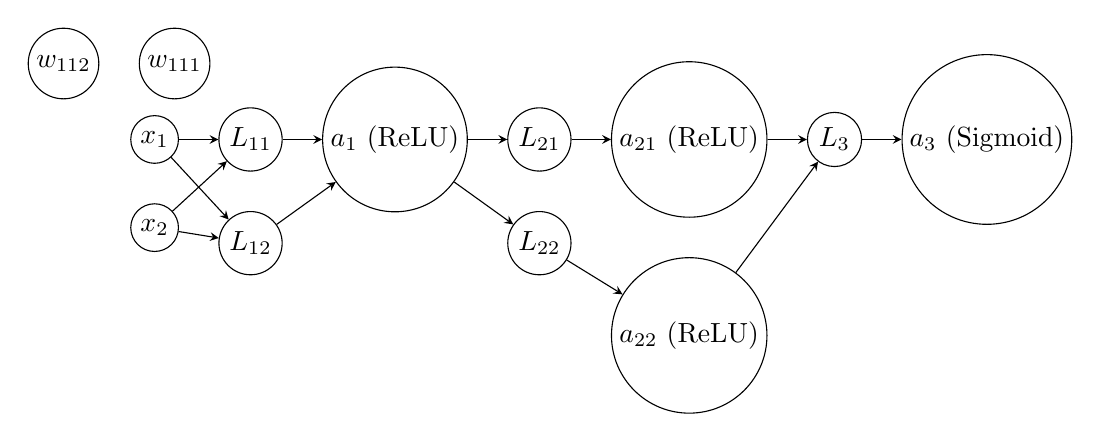
\begin{tikzpicture}[%
    activation/.style={%
        draw,
        circle,
        inner sep=2pt,
        minimum size=0.5cm,
        node distance=0.5cm
    },
    input/.style={%
        draw,
        circle,
        inner sep=2pt,
        minimum size=0.5cm,
        node distance=0.5cm
    },
    inputLayer/.style={%
        draw,
        circle,
        inner sep=2pt,
        minimum size=0.5cm,
        node distance=0.5cm
    },
    hidden/.style={%
        draw,
        circle,
        inner sep=2pt,
        minimum size=0.5cm,
        node distance=0.5cm
    },
    output/.style={%
        draw,
        circle,
        inner sep=2pt,
        minimum size=0.5cm,
        node distance=0.5cm
    },
    >=stealth
]

% Inputs
\node[input] (input1) {$x_1$};
\node[input, below=of input1] (input2) {$x_2$};

% Input layer 1 (L_1)
\node[inputLayer, right=of input1] (inputLayer1) {$L_{11}$};
\node[inputLayer, below=of inputLayer1] (inputLayer2) {$L_{12}$};
\node[inputLayer, above left=of inputLayer1] (inputWeight1) {$w_{111}$};
\node[inputLayer, left=of inputWeight1] (inputWeight2) {$w_{112}$};

% Input Layer Activation
\node[activation, right=of inputLayer1] (activation1) {$a_{1}$ (ReLU)};

% Hidden layer 2 (L_2)
\node[hidden, right=of activation1] (hidden1) {$L_{21}$};
\node[hidden, below=of hidden1] (hidden2) {$L_{22}$};

% Hidden Layer Activation
\node[activation, right=of hidden1] (activation21) {$a_{21}$ (ReLU)};
\node[activation, below=of activation21] (activation22) {$a_{22}$ (ReLU)};

% Output layer (L_3)
\node[output, right=of activation21] (output1) {$L_{3}$};

% Output Layer activation
\node[activation, right=of output1] (activation3) {$a_{3}$ (Sigmoid)};

% Arrows
\draw[->] (input1) -- (inputLayer1);
\draw[->] (input1) -- (inputLayer2);
\draw[->] (input2) -- (inputLayer1);
\draw[->] (input2) -- (inputLayer2);

\draw[->] (inputLayer1) -- (activation1);
\draw[->] (inputLayer2) -- (activation1);

\draw[->] (activation1) -- (hidden1);
\draw[->] (activation1) -- (hidden2);


\draw[->] (hidden1) -- (activation21);
\draw[->] (hidden2) -- (activation22);

\draw[->] (activation21) -- (output1);
\draw[->] (activation22) -- (output1);

\draw[->] (output1) -- (activation3);

\end{tikzpicture}

\end{document}
